\documentclass[border=8pt]{standalone}
\usepackage[T1]{fontenc}
\usepackage{helvet}
\renewcommand{\familydefault}{\sfdefault}
\usepackage{tikz}
\usetikzlibrary{shapes.geometric, arrows.meta, positioning, calc, fit, backgrounds}

% ── Colour palette ──────────────────────────────────────────────
\definecolor{navy}{HTML}{002D40}
\definecolor{cred}{HTML}{D61F39}
\definecolor{amber}{HTML}{E6A740}
\definecolor{slate}{HTML}{82979F}
\definecolor{dgrey}{HTML}{4C4D4E}
\definecolor{initbg}{HTML}{EDF0F2}
\definecolor{stage1bg}{HTML}{E8F0F3}
\definecolor{stage2bg}{HTML}{FDF5E6}

% ── Node styles ─────────────────────────────────────────────────
\tikzset{
  process/.style={
    rectangle, rounded corners=3pt,
    minimum width=46mm, minimum height=8mm,
    text width=44mm, align=center,
    draw=navy, line width=0.6pt, fill=white,
    font=\scriptsize\sffamily, text=dgrey,
  },
  decision/.style={
    diamond, aspect=2.2,
    minimum width=36mm, minimum height=10mm,
    text width=24mm, align=center,
    draw=navy, line width=0.6pt, fill=white,
    font=\scriptsize\sffamily, text=dgrey,
    inner sep=1pt,
  },
  terminal/.style={
    rectangle, rounded corners=5pt,
    minimum width=22mm, minimum height=7mm,
    text width=20mm, align=center,
    draw=#1, line width=0.8pt, fill=#1!8,
    font=\scriptsize\bfseries\sffamily, text=#1,
  },
  terminal/.default=navy,
  annot/.style={font=\tiny\sffamily, text=slate},
  arr/.style={
    -{Stealth[length=2.2mm, width=1.6mm]},
    line width=0.5pt, color=dgrey,
  },
  darr/.style={
    -{Stealth[length=2.2mm, width=1.6mm]},
    line width=0.5pt, color=slate, dashed,
  },
  stagelabel/.style={font=\footnotesize\bfseries\sffamily, text=navy},
  substep/.style={
    rectangle, rounded corners=2pt,
    minimum width=46mm, minimum height=7mm,
    text width=44mm, align=center,
    draw=slate, line width=0.4pt, fill=white,
    font=\scriptsize\sffamily, text=dgrey,
  },
  iterbox/.style={
    rectangle, rounded corners=2pt,
    minimum width=46mm, minimum height=7mm,
    text width=44mm, align=center,
    draw=amber!80!black, line width=0.5pt, fill=amber!6,
    font=\scriptsize\sffamily, text=dgrey,
  },
}

\begin{document}
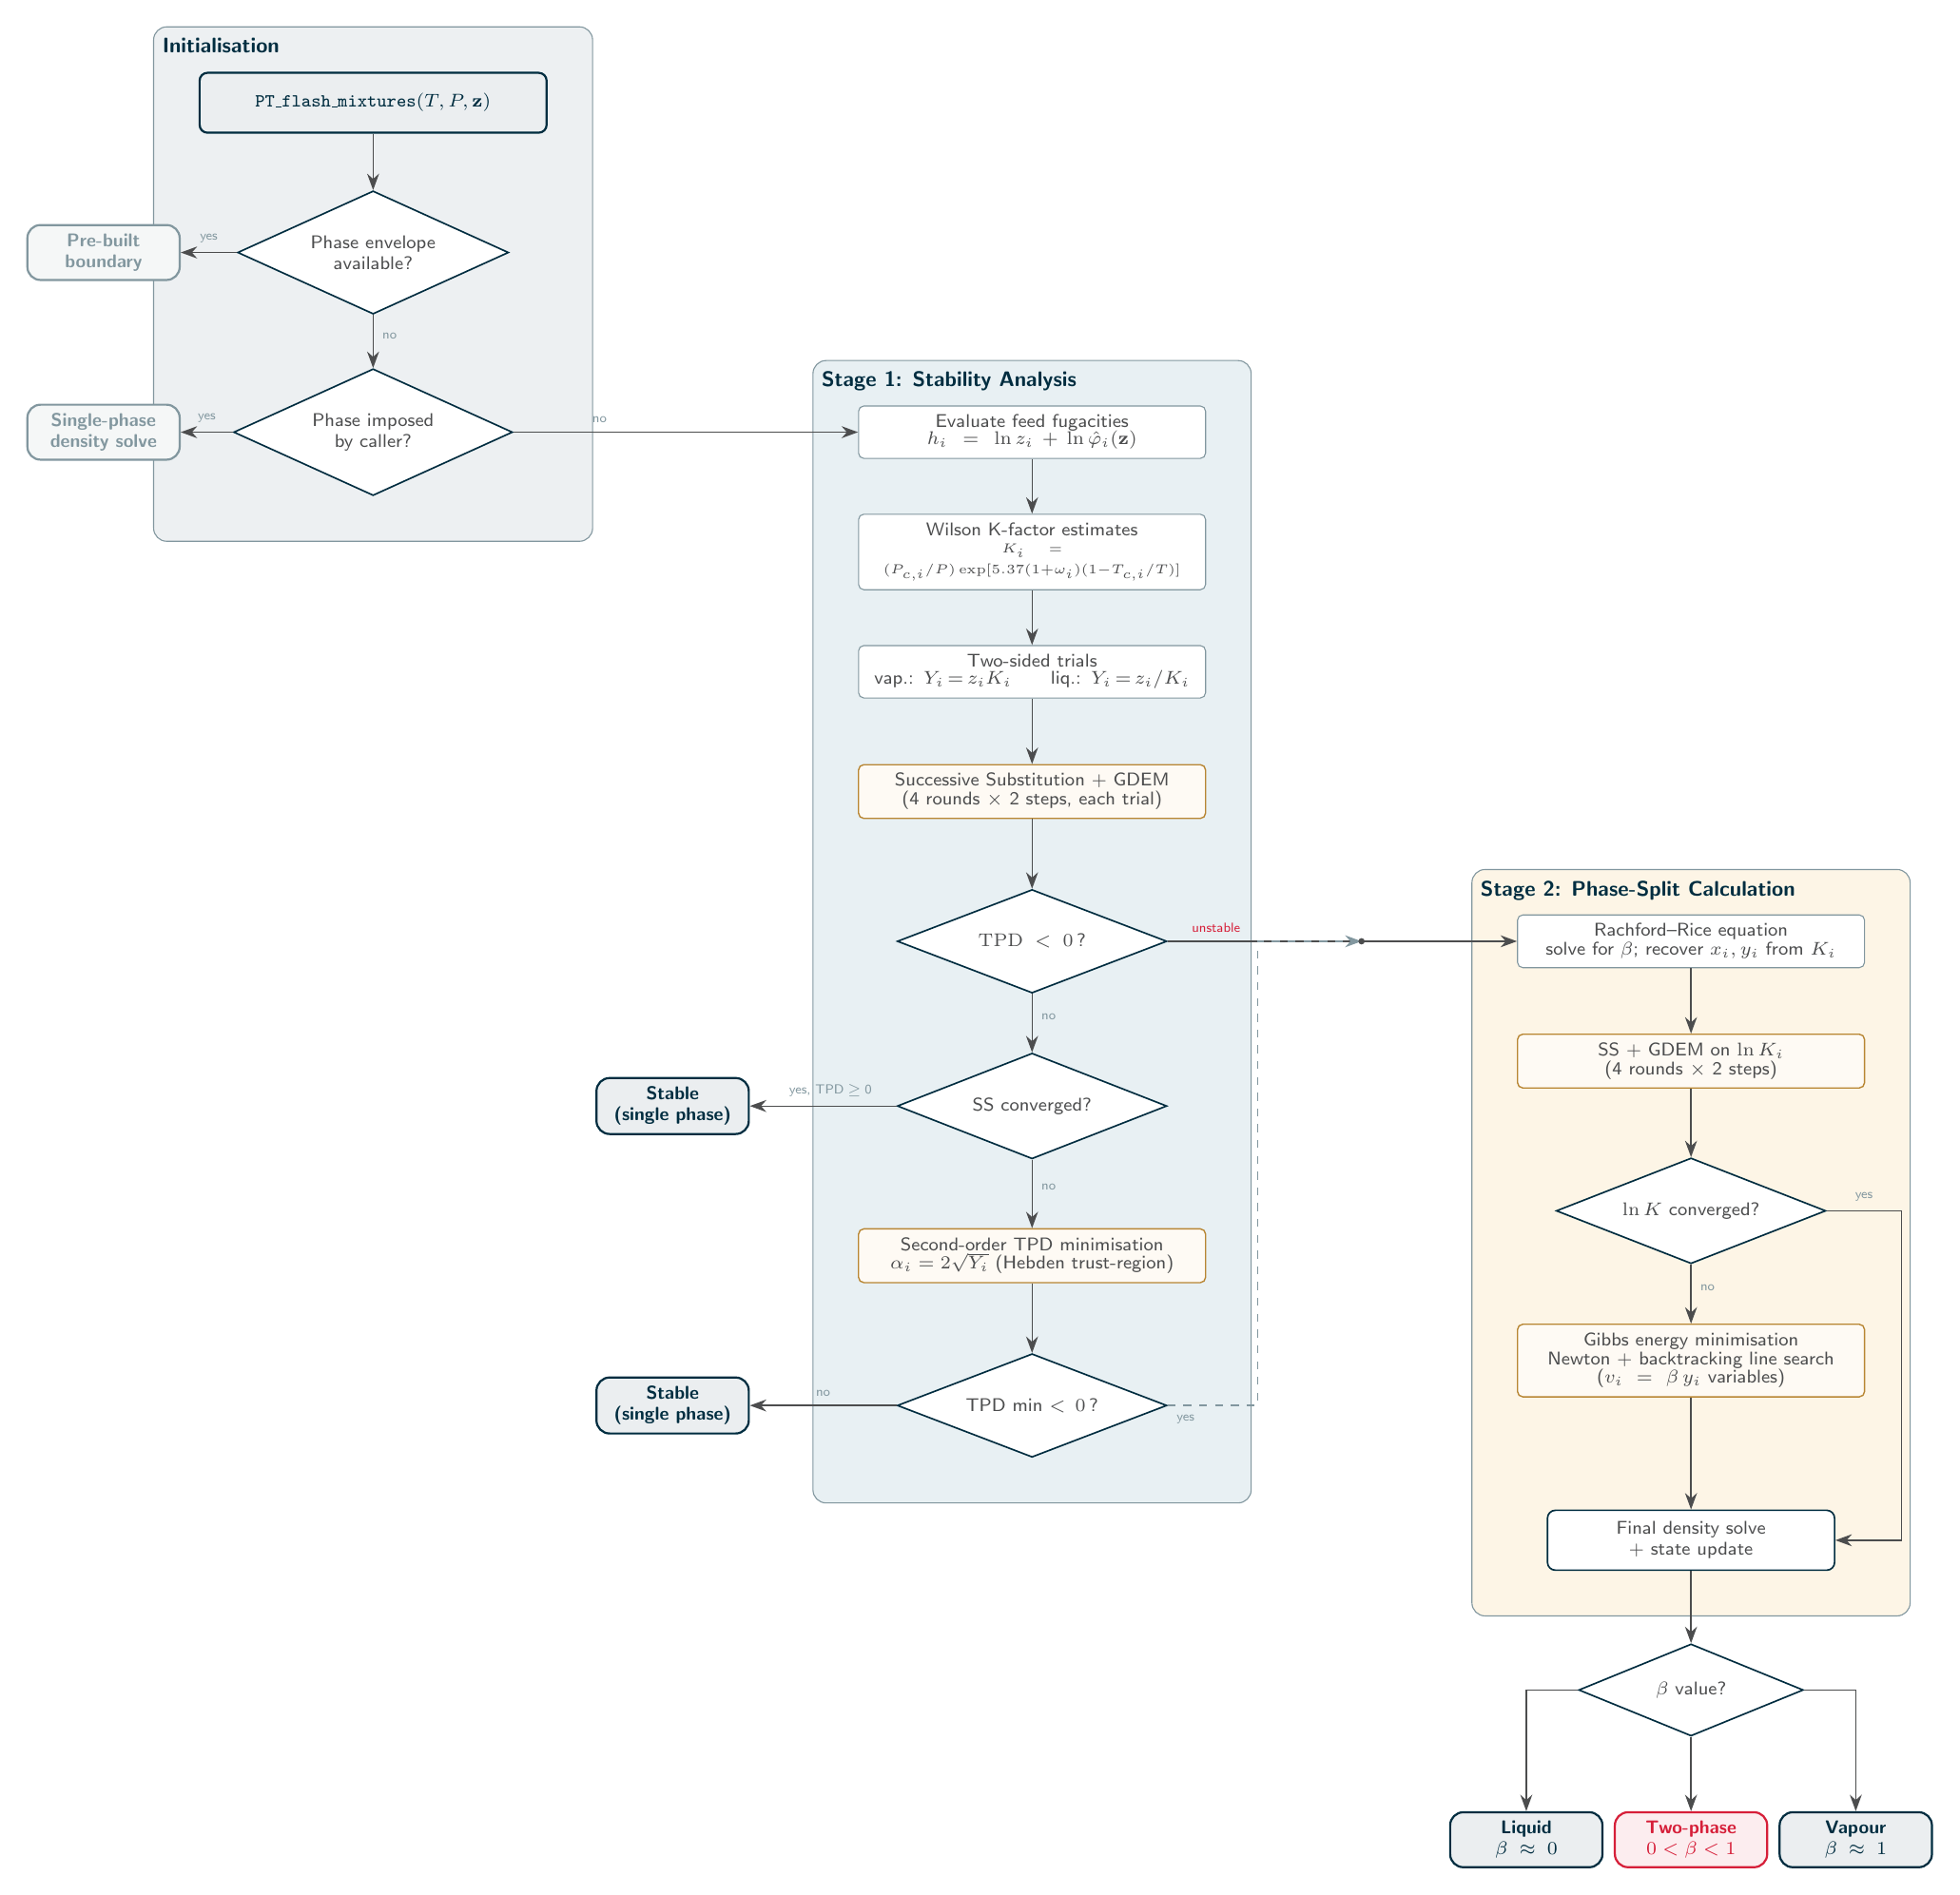
\begin{tikzpicture}

% ════════════════════════════════════════════════════════════════
% COLUMN 1 — INITIALISATION  (centred at x = 0)
% ════════════════════════════════════════════════════════════════
\node[process, fill=navy!8, draw=navy, line width=0.8pt,
      font=\scriptsize\bfseries\sffamily, text=navy]
  at (0,0) (entry) {\texttt{PT\_flash\_mixtures}$(T,P,\mathbf{z})$};

\node[decision] at (0,-20mm) (d_env) {Phase envelope\\available?};
\draw[arr] (entry) -- (d_env);

\node[terminal=slate, minimum width=20mm, text width=18mm]
  at (-36mm,-20mm) (env_exit) {Pre-built\\boundary};
\draw[arr] (d_env.west) -- node[annot, above] {yes} (env_exit);

\node[decision] at (0,-44mm) (d_imp) {Phase imposed\\by caller?};
\draw[arr] (d_env.south) -- node[annot, right, pos=0.4] {no} (d_imp);

\node[terminal=slate, minimum width=20mm, text width=18mm]
  at (-36mm,-44mm) (imp_exit) {Single-phase\\density solve};
\draw[arr] (d_imp.west) -- node[annot, above] {yes} (imp_exit);

% ════════════════════════════════════════════════════════════════
% COLUMN 2 — STAGE 1: STABILITY ANALYSIS  (centred at x = 88mm)
% Top node aligned with d_imp so the "no" arrow is horizontal.
% ════════════════════════════════════════════════════════════════
\node[substep] at (88mm, -44mm) (feed_fug)
  {Evaluate feed fugacities\\[-0.5mm]
   $h_i = \ln z_i + \ln\hat\varphi_i(\mathbf{z})$};

\node[substep] at (88mm, -60mm) (wilson)
  {Wilson K-factor estimates\\[-0.5mm]
   {\tiny $K_i = (P_{c,i}/P)\exp[5.37(1{+}\omega_i)(1{-}T_{c,i}/T)]$}};

\node[substep] at (88mm, -76mm) (trials)
  {Two-sided trials\\[-0.5mm]
   vap.: $Y_i\!=\!z_i K_i$\qquad liq.: $Y_i\!=\!z_i/K_i$};

\node[iterbox] at (88mm, -92mm) (ss_gdem)
  {Successive Substitution + GDEM\\[-0.3mm]
   (4 rounds $\times$ 2 steps, each trial)};

\node[decision] at (88mm, -112mm) (d_tpd1) {$\mathrm{TPD} < 0$\,?};

\node[decision] at (88mm, -134mm) (d_conv) {SS converged?};

\node[iterbox] at (88mm, -154mm) (tpd_min)
  {Second-order TPD minimisation\\[-0.3mm]
   $\alpha_i\!=\!2\sqrt{Y_i}$ (Hebden trust-region)};

\node[decision] at (88mm, -174mm) (d_tpd2) {TPD min $< 0$\,?};

% Stage 1 vertical spine
\draw[arr] (feed_fug) -- (wilson);
\draw[arr] (wilson) -- (trials);
\draw[arr] (trials) -- (ss_gdem);
\draw[arr] (ss_gdem) -- (d_tpd1);
\draw[arr] (d_tpd1.south) -- node[annot, right, pos=0.4] {no} (d_conv);
\draw[arr] (d_conv.south) -- node[annot, right, pos=0.4] {no} (tpd_min);
\draw[arr] (tpd_min) -- (d_tpd2);

% Stable exits → LEFT (between Init and Stage 1)
\node[terminal=navy, minimum width=20mm, text width=18mm]
  at (40mm, -134mm) (stable1) {Stable\\(single phase)};
\draw[arr] (d_conv.west) -- node[annot, above, pos=0.45]
  {yes, TPD$\,{\geq}\,$0} (stable1);

\node[terminal=navy, minimum width=20mm, text width=18mm]
  at (40mm, -174mm) (stable2) {Stable\\(single phase)};
\draw[arr] (d_tpd2.west) -- node[annot, above] {no} (stable2);

% ════════════════════════════════════════════════════════════════
% COLUMN 3 — STAGE 2: PHASE-SPLIT CALCULATION (centred at x = 176mm)
% Top node aligned with d_tpd1 so the "unstable" arrow is horizontal.
% ════════════════════════════════════════════════════════════════
\node[substep] at (176mm, -112mm) (rr)
  {Rachford--Rice equation\\[-0.3mm]
   solve for $\beta$; recover $x_i, y_i$ from $K_i$};

\node[iterbox] at (176mm, -128mm) (ss2)
  {SS + GDEM on $\ln K_i$\\[-0.3mm]
   (4 rounds $\times$ 2 steps)};

\node[decision] at (176mm, -148mm) (d_ss2) {$\ln K$ converged?};

\node[iterbox] at (176mm, -168mm) (gibbs)
  {Gibbs energy minimisation\\[-0.3mm]
   Newton + backtracking line search\\[-0.3mm]
   ($v_i\!=\!\beta\,y_i$ variables)};

\node[process, minimum width=38mm, text width=36mm]
  at (176mm, -192mm) (final_update)
  {Final density solve\\+ state update};

% Stage 2 vertical spine
\draw[arr] (rr) -- (ss2);
\draw[arr] (ss2) -- (d_ss2);
\draw[arr] (d_ss2.south) -- node[annot, right, pos=0.4] {no} (gibbs);
\draw[arr] (gibbs) -- (final_update);

% Yes bypass: d_ss2 → final_update (route right of spine)
\draw[arr] (d_ss2.east) -- node[annot, above] {yes} ++(10mm,0)
  |- (final_update.east);

% Result classification
\node[decision, minimum width=30mm, text width=20mm]
  at (176mm, -212mm) (d_beta) {$\beta$ value?};
\draw[arr] (final_update) -- (d_beta);

\node[terminal=navy, minimum width=20mm, text width=18mm]
  at (154mm, -232mm) (res_liq) {Liquid\\$\beta \approx 0$};
\node[terminal=cred, minimum width=20mm, text width=18mm]
  at (176mm, -232mm) (res_2ph) {Two-phase\\$0\!<\!\beta\!<\!1$};
\node[terminal=navy, minimum width=20mm, text width=18mm]
  at (198mm, -232mm) (res_vap) {Vapour\\$\beta \approx 1$};

\draw[arr] (d_beta.west) -| (res_liq);
\draw[arr] (d_beta.south) -- (res_2ph);
\draw[arr] (d_beta.east) -| (res_vap);

% ════════════════════════════════════════════════════════════════
% CROSS-COLUMN CONNECTIONS
% ════════════════════════════════════════════════════════════════

% Init "no" → Stage 1 (horizontal, same y = -44mm)
\draw[arr] (d_imp.east) -- node[annot, above, pos=0.25] {no} (feed_fug.west);

% Stage 1 → Stage 2: d_tpd1 "yes" (horizontal, same y = -112mm)
\coordinate (s2merge) at (132mm, -112mm);
\draw[arr] (d_tpd1.east) -- node[annot, above, pos=0.25]
  {\textcolor{cred}{unstable}} (s2merge) -- (rr.west);

% Stage 1 → Stage 2: d_tpd2 "yes" (routes right then up to merge)
\draw[darr] (d_tpd2.east) -- node[annot, below, pos=0.2] {yes}
  ++(12mm,0) |- (s2merge);
\fill[dgrey] (s2merge) circle (1.2pt);

% ════════════════════════════════════════════════════════════════
% BACKGROUND BOXES
% ════════════════════════════════════════════════════════════════
\begin{scope}[on background layer]
  % Init box
  \node[fit=(entry)(d_env)(d_imp),
        rounded corners=5pt, fill=initbg, draw=slate,
        line width=0.4pt, inner sep=6mm] (initbox) {};
  % Stage 1 box
  \node[fit=(feed_fug)(wilson)(trials)(ss_gdem)
        (d_tpd1)(d_conv)(tpd_min)(d_tpd2),
        rounded corners=5pt, fill=stage1bg, draw=slate,
        line width=0.4pt, inner sep=6mm] (s1box) {};
  % Stage 2 box
  \node[fit=(rr)(ss2)(d_ss2)(gibbs)(final_update),
        rounded corners=5pt, fill=stage2bg, draw=slate,
        line width=0.4pt, inner sep=6mm] (s2box) {};
\end{scope}

% Stage labels
\node[stagelabel, anchor=north west] at (initbox.north west)
  {\strut Initialisation};
\node[stagelabel, anchor=north west] at (s1box.north west)
  {\strut Stage 1: Stability Analysis};
\node[stagelabel, anchor=north west] at (s2box.north west)
  {\strut Stage 2: Phase-Split Calculation};

\end{tikzpicture}
\end{document}
